\documentclass[paper=a4,fontsize=12pt,ngerman]{scrartcl}

\usepackage[utf8]{inputenc}				
\usepackage[T1]{fontenc}
\usepackage{graphicx}
\usepackage[ngerman]{babel}
\usepackage{amssymb}
\usepackage{amsmath}
\usepackage[a4paper,left=25mm,right=35mm,top=25mm,bottom=30mm]{geometry}
\usepackage{parskip}
\usepackage{listings}
\usepackage{xcolor}
\usepackage{float}
\usepackage{adjustbox}  % Add this to your preamble
\lstset{
  language=Python,
  basicstyle=\ttfamily\small,
  keywordstyle=\color{blue},
  stringstyle=\color{red},
  commentstyle=\color{green!50!black},
  showstringspaces=false,
  numbers=left,
  numberstyle=\tiny\color{gray},
  frame=single,
  breaklines=true
}

\begin{document}

\pagenumbering{roman}
\pagestyle{plain}

% Einbinden der Titelseite
\begin{titlepage}

\linespread{1.5}


\includegraphics[width=\linewidth]{graphics/htw_logo}

\begin{center}
    \large  
    \hfill
    \vfill
    \Large{\bfseries{Audioverarbeitung mittels eines Computers}}
    
    von \\
    Amsakan Bavan \\
    Matrikelnummer: 5011657

    \vfill
		
    Ein wissenschaftlicher Bericht im Rahmen der Vorlesung\\
    \glqq Wissenschaftliches Arbeiten\grqq\\
    an der htw saar im Studiengang Informatik\\
	
    \vfill	
    \vfill
	
    Saarlouis, den 18.08.2025
\end{center}
    
\end{titlepage}


% Hier ist der Abstract
\section*{Abstract}
In dieser Arbeit befassen wir uns mit der Audioverarbeitung von Computern. Dabei definieren wir einige Grundlagen und Begriffe der Audioverarbeitung und der
digitalen Signalverarbeitung. Außerdem betrachten wir einige bestehende Lösungen
zur Audiokomprimierung und Audiobearbeitung. Außerdem vergleichen wir diese
Audiokomprimierungslösungen. Daüber hinaus beleuchten wir theoretische Konzepte der digitalen Signalverarbeitung und Operationen wie die diskrete FourierTransformation und Faltung werden erklärt. Danach wird das theoretische Konzept
der diskreten Fourier-Transformation implementiert, welche wir dann verwenden um
ein eigenes Audioverarbeitungsprogramm zu implementieren.

\newpage
\section*{Selbstständigkeitserklärung}
Ich versichere, dass ich die vorliegende Arbeit selbstständig verfasst und 
keine anderen als die angegebenen Quellen und Hilfsmittel benutzt habe.
Insbesondere habe ich alle KI-basierten Werkzeuge angegeben, die ich bei
der Erstellung, Übersetzung oder Überarbeitung des Textes verwendet habe.

Ich erkläre hiermit weiterhin, dass die vorgelegte Arbeit zuvor weder von mir 
noch von einer anderen Person an dieser oder einer anderen Hochschule 
eingereicht wurde.

Darüber hinaus ist mir bekannt, dass die Unrichtigkeit dieser Erklärung eine 
Benotung der Arbeit mit der Note \glqq nicht ausreichend\grqq \ zur Folge hat 
und einen Ausschluss von der Erbringung weiterer Prüfungsleistungen zur Folge 
haben kann.
\bigskip
 
Saarlouis, den 18.08.2025





% Das Inhaltsverzeichnis
\clearpage
\tableofcontents 

\clearpage
\pagenumbering{arabic}

% Hier beginnt das erste Kapitel
\section{Einleitung}
In der heutigen Zeit, ermöglichen Programme wie Konferenzsoftware, Digitale Audio Workstations, Aufnahmeprogramme, Messagingprogramme und viele mehr, die
Möglichkeit Töne, Sprache und Geräusche zu verarbeiten. Dies ist möglich dank
digitaler Signalverarbeitung kombiniert mit Echtzeitlösungen wie Ringpuffern, Pufferung und vielem mehr. In diesem Dokument beleuchten wir einige bestehende
Lösungen, welche die Audioverarbeitung auf Computern ermöglichen. Außerdem betrachten wir die Theorie der digitalen Signalverarbeitung und schauen uns auch die
Implementierungen von diesen theoretischen Komzepten an. Darüber hinaus implementieren wir ein einfaches Audioverarbeitungsprogramm, welches eine Audiodatei
annimmt und eine Filtrierung durch Fourier-Analyse vornimmt. Unter der Audiovearbeitung definieren wir die Komprimierung, Bearbeitung und Übertragung eines
bestehenden Audiosignals.


\subsection{Grundlagen und Begriffe}

Bevor wir in das Thema einleiten, werden einige grundlegende Begriffe aus der Signal- und Audioverarbeitung erläutert:

\textbf{Audioverarbeitung}
Unter der Audioverarbeitung definieren wir die Komprimierung, Bearbeitung und
Übertragung eines bestehenden Audiosignals.

\textbf{Audiobearbeitung}
Die Audiobearbeitung dient dazu, das Bearbeitungen an einem Audiosignal vorgenommen werden können. Einige Beispiele für solche Bearbeitungen sind Verzerrung,
das Filtrieren von Frequenzbereichen (oder auch Frequenzbändern), das Anwenden
eines Halleffektes oder auch das Verstellen bei der Audioaufnahme eines Musikstückes.

\textbf{Puls-Code-Modulation}
"Pulse code modultion (PCM) embodies the basic concepts of transmitting a sequence of symbols, i.e., pulses to represent information." \cite{waggener1995pulse} (Seite 7, Abschnitt 1)

\textbf{Abtrastrate}
Die Abtastrate oder auch Abtastfrequenz bezeichnet die Anzahl an Abtastwerten
pro Sekunde. \cite{knapp2023bituebertragung, oppenheim2013discrete}

\textbf{Bittiefe}
Die Bittiefe beschreibt die Anzahl an bits, welche pro Abtastwert hinterlegt werden. \cite{knapp2023bituebertragung, oppenheim2013discrete}

\textbf{Codec}
Codec ist die Kurzschreibweise für "Coder Decoder". Bei einem Codec wird das
digitalisierte Audiosignal durch einen Kodierer gemäss eines gegebenen Formates
kodiert (und bei komprimierten Codecs auch komprimiert). Diese kodierten und
komprimierten Audiodaten kann man übertragen oder auch abspeichern und durch
die Dekodierung dieses Signals, erhält man je nach Codec das Signal entweder in
voller Gänze oder eine Annäherung davon (beispielsweise bei verlustbehafteter Audiokompression).

\label{BL}
\section{Bestehende Lösungen}
Gemäß der Definition der Audioverarbeitung gibt es schon einige bestehende Lösungen für diese:

\subsection{Bestehe Lösungen zur Audiokomprimierung}
Die Audiokomprimierung dient dazu, dass ein digitalisiertes AUdiosignal in dessen Bandbreite zu komprimieren, um diese zur Übertragung, Abspericherung oder Weiterverarbitung schneller und einfacher handzuhaben. 
Das analoge Audiosignal wird durch Pulsweitenmodulation abgetastet und digitaliert. 
Dabei haben die Abtastparameter, wie Abtrastrate und Bittiefe eine große Auswirkung auf der Bandbreite des digitalisierten Signals.
Die Standardwerte für ein Musikstück beispielsweise sind eine Abtraste von 44.100 kHz und eine Bittiefe von 24 Bit. 
Hierbei bewegt man sich in den Größenbereichen von 20 Megabyte bis 60 Megabyte. 
Diese Größen sind nicht leicht handhabbar für die Übertragung oder gar beispielsweise für die Abspericherung auf mobilen Endgeräte.
Umegesetzt wird das ganze durch Codecs. Dabei muss man unterscheiden zwischen verlustfreien und verlustbehafteten Codecs.

Beispiele für verlustfreie Codecs sind die folgenden \cite{gzmk}

\begin{enumerate}
    \item Free Lossless Audio Codec (kurz \textbf{FLAC}) \cite{rfc9639}
    \item Wavpack \cite{kurtisi2008wavpack}
    \item Apple Lossless Audio Codec (kurz \textbf{ALAC})
    \item Monkey’s Audio
    \item True Audio
\end{enumerate}

Beispiele für verlustbehaftete Codecs hingegen sind:

\begin{enumerate}
    \item MPEG Audio Layer 3
    \item Vorbis
\end{enumerate}


Diese Lösungen werden je nach Anwendungsfall in heutiger Software, welche Audio benötigen weitesgehend verwendet.

\subsection{Bestehende Lösungen zur Audiobearbeitung}

Meist werden für die Audiobearbeitung digitale Audio Workstations verwendet. 
Einige Beispiele für solche digitalen Audio Workstations sind:

\begin{itemize}
    \item Ableton Live
    \item FL Studio
    \item Bitwig Studio
    \item Cockos Reaper
\end{itemize}

\begin{figure}[H]
    \centering
    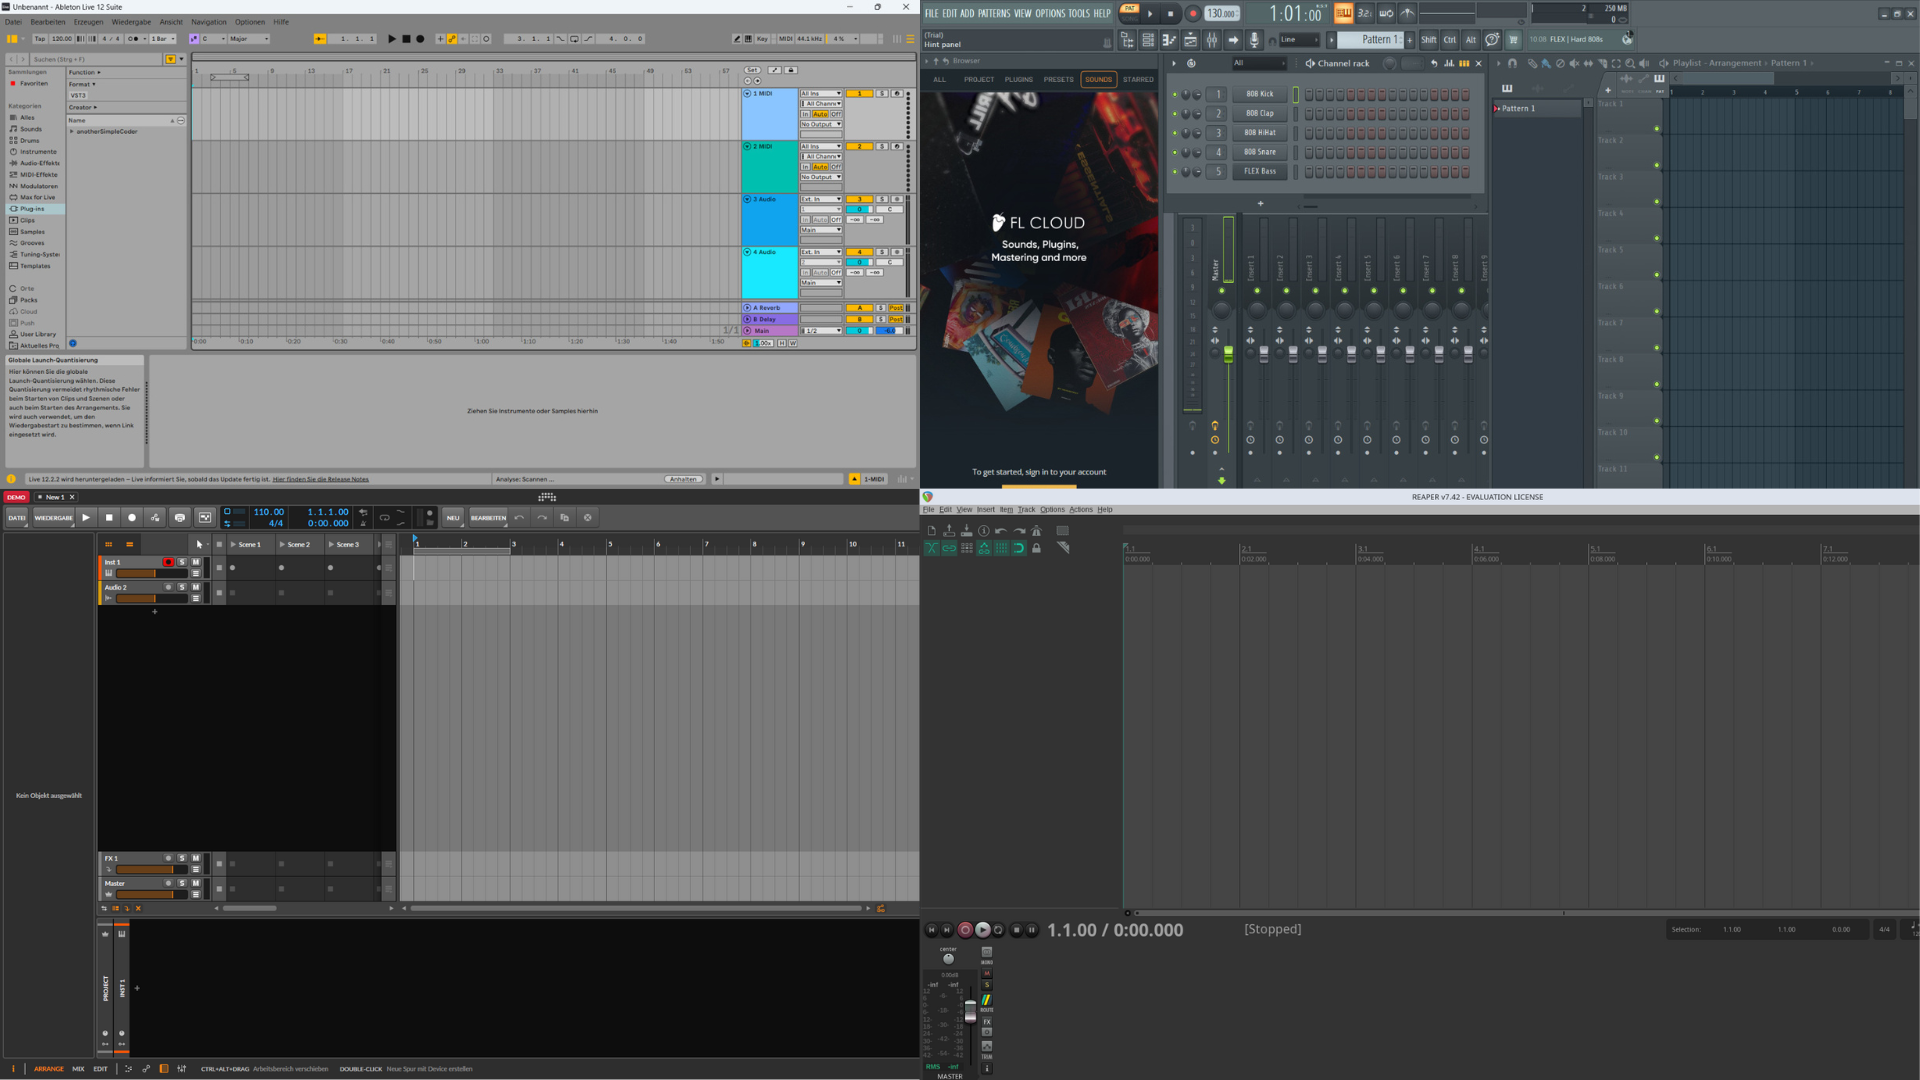
\includegraphics[width=0.8\textwidth]{graphics/DAWs.png}
    \caption{Eine Übersicht der oben genannten digitalen Audio Workstations.}
\end{figure}


\section{Theorie}

Damit die in \ref{BL} angegebenen Lösungen umgesetzt werden können, müssen entsprechende theoretische Grundlagen, dem Rechner vorgelegt werden.
Im Falle der Audioverarbeitung basieren diese theoretischen Grundlagen auf der digitalen Signalverarbeitung.

\subsection{Digitale Signalverarbeitung}

Nach Steven W. Smith: "Digital Signal Processing is distinguished from other areas
in computer science by the unqiue type of data it uses: signals. In most cases, these signals originate as sensory data from the real world: seismic vibrations, visual
images, sound waves, etc. DSP is the mathematics, the algorithms and the techniques used to manipulate these signals after they have been concerted into a digital
form."\cite{sws1} (Seite 1 Abschinitt 2)

In dieser Arbeit betrachten wir zwei Algorithmen aus der digitalen Signalverarbeitung. Zum einen die diskrete Fourier-Transformation und zum anderen die Faltung.

\subsection{Die diskrete Fourier-Transformation}

"The Discrete Fourier Transform (DFT) is the equivalent of the continuous Fourier
Transform for signals known only at instants separated by sample times (i.e.
a finite sequence of data)"\cite{roberts_dft_slides} (Seite 141 Abschnitt 1)

Dadurch erhält man neben der Zeit-Amplituden Repräsentation nun eine Amplituden-Frequnz Repräsentation des Signals, wodurch es möglich ist Bearbeitungen wie die Filtrierung von Frequenzbereichen eines Audiosignals vorzunehmen.
Man spricht hierbei auch von einer Konvertierung von der Zeitdomöne zur Frequenzdomäne.

\begin{figure}[H]
    \centering
    \includegraphics[width=0.8\textwidth]{graphics/amplitudenDarstellung.pdf}
    \caption{Amplitudendarstellung des Stücks "Beethoven Symphony No.9 (Scherzo)"}
    \label{fig:scherzo-amplitude}
\end{figure}

\begin{figure}[H]
    \centering
    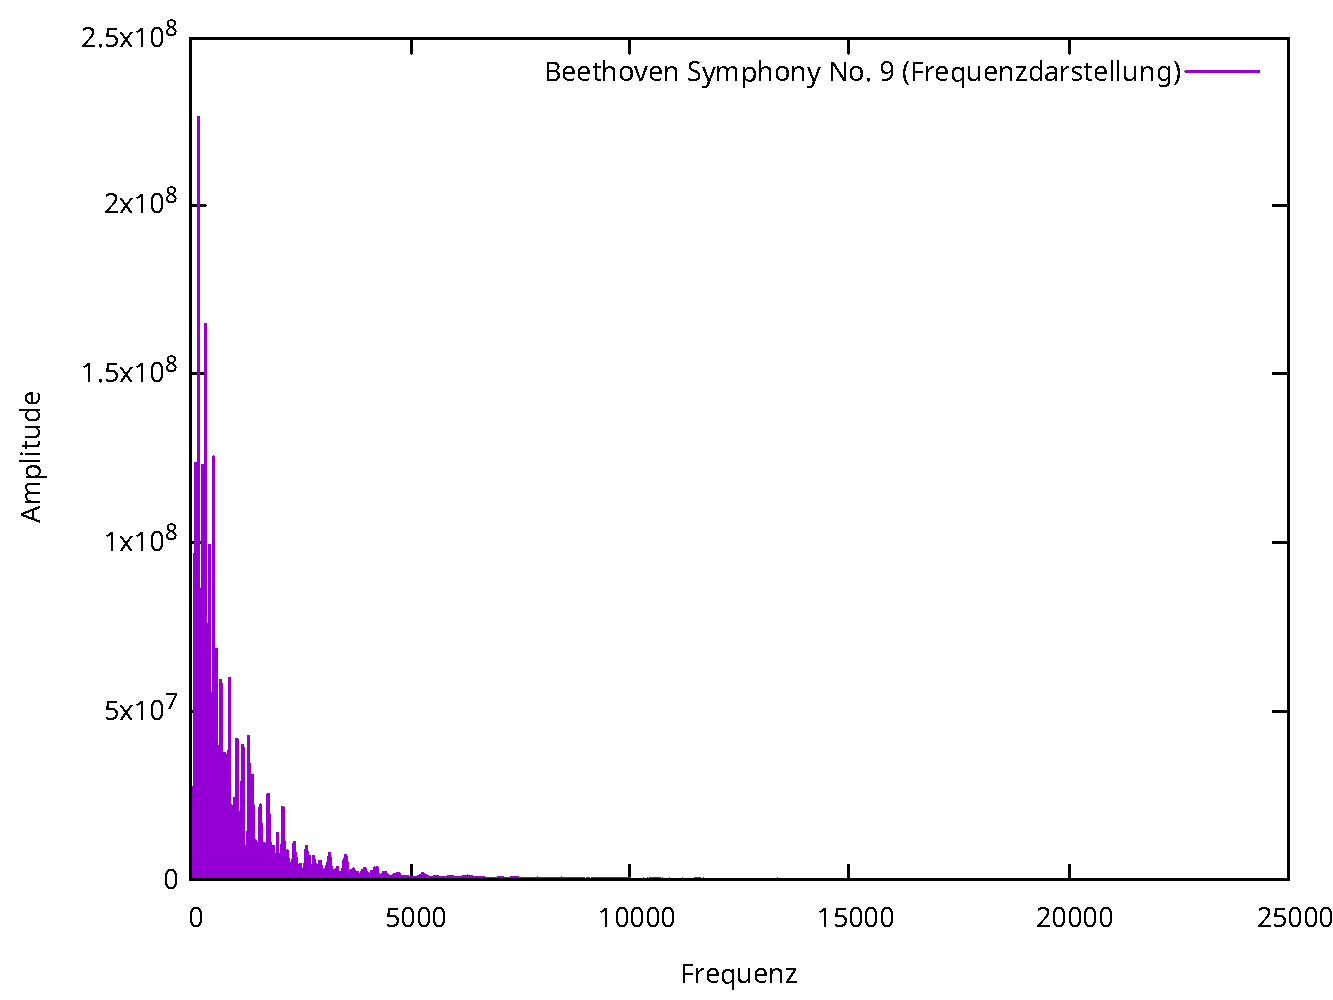
\includegraphics[width=0.8\textwidth]{graphics/frequnzDarstellung.pdf}
    \caption{Frequenzdarstellung des Stücks "Beethoven Symphony No.9 (Scherzo)"}
    \label{fig:scherzo-frequenz}
\end{figure}

Bei der diskreten Fourier Transformation wird dabei wie folgt vorgegangen:

Gegeben sei ein kontinuierliches Signal, dargestellt durch eine komplexe Funktion $f(t)$, wobei $t$ die Zeit beschreibt. Dabei tasten wir dieses Signal ab und erhalten damit eine endliche Anzahl an $N \in \mathbb{N}$ Messpunkten in einem Abstand $T \in \mathbb{N}$. Diese notieren wir mit $f[0], f[1],$ \dots $f[N+1]$.

Die Fourier-Transformation des ursprünglichen Signals $f(t)$ wäre dabei

$$F(j \omega) =\int_{-\infty}^{\infty} f(t)e^{-j\omega t} dt $$

Dadurch, dass wir abei mit einem diskreten Signal arbeiten, welches aus einzelnen Messpunkten bestehen, verändert sich unser diskretes Integral wie folgt:

$$F(j\omega) = \int_0^{(N-.1)T} f(t)e^{-j\omega t}$$
$$= f[0]e^{j0} + f[1]e^{-j\omega T} + \dots + f[N-1]e^{-j\omega (N-1) T}$$

\cite{roberts_dft_slides}

oder auch

$$F(j\omega) = \sum_{k=0}^{N-1} f[k]e^{-j\omega kT}$$

$F(j\omega)$ liefert uns dabei für eine Frequenz $\omega$ dessen Amplitudenanteil in dem Signal und $j$ ist die imaginäre Zahl in $\mathbb{C}$.

$$\omega \in \{0, \frac{2\pi}{NT}, \frac{2\pi}{NT} \cdot 2, \dots, \frac{2\pi}{NT} \cdot (N-1)\}$$

\cite{roberts_dft_slides}

Aus all dem ergibt sich die folgende Formel für die diskrete Fourier-Transformation:

$$F[n] = \sum_{k=0}^{N-1} f[k]e^{-j\frac{2\pi}{N}nk} (n=0 : N-1)$$

\cite{roberts_dft_slides}

\subsection{Faltung}

Bei der Faltung handelt es sich neben der diskreten Fourier-Transformation auch um eine Operation aus der digitalen Signalverarbeitung. Dabei werden zwei Signale 
$f$ und $g$ zusammengeführt. Mathematisch lässt sich diese Zusammenführung wie folgt beschreiben:

Sei $h$ die Faltungsfunktion \cite{dolequez}:

$$g(n) = \sum_{k} f(k) h(n-k) = \sum_{k} h(k) x (n-k)$$

Die Faltung findet sehr oft Verwendung in der Audiobearbeitung, um Halleffekte anhand eines gegeben Raumhallsignales zu realisieren. Diese Effekte nennt man auch
entsprechend Faltungshall.

\section{Implementierung der diskreten Fourier-Transformation}

Dadurch, dass wir nun einige theoretische Grundlagen der Audioverarbeitung festgelegt haben, können wir diese nun implementieren. Dabei setzen wir den Fokus auf der diskreten Fourier-Transformation, da 
diese in der Audioverarbeitung am relevantesten ist und in vielerlei Audioverarbeitungssoftware Verwendung findet.

Der Pseduocode zur Implementierung der diskreten Fourier Transformation sieht wie folgt aus:

\begin{lstlisting}
    def discrete_fourier_transform(signal, samples):
        result = list()

        for k in range(0, N):
            sum = 0
            for n in range(0, N):
                angle = (-2 * PI * k * n) / N
            result.push(sum)
\end{lstlisting}

\section {Eigenimplementierung eines Audioverarbeitungsprogramms}

Nachdem wir mit der Implementierung der diskreten Fourier Transformation nun eine der wichtigsten Operationen der Audioverarbeitung implementiert haben, versuchen wir uns nun an der Implementierung eines vollwertigen Audioprogrammes.
In der Audiosoftwareindustrie ist es dabei üblich, dass auf Programmiersprachen wie C, C++ oder auch Rust gesetzt werden. In dieser Arbeit findet die Implementierung in C++ statt, da diese am weitesten verbreitet ist zur Entwicklung von
Audioverarbeitungsapplikationen mit der Begrüdung, dass hier auch durch direkter Ausführung auf der Hardware, die nötigen Resourcen zur Audioverarbeitung verwendet werde mit möglichst geringer Latenz.

Das Audioverarbeitungsprogramm was wir implementieren werden läuft auf der Kommandozeile und nimmt eine Audiodatei im RIFF-WAVE Format an.
Über einen Kommandozeilenparameter wird die Frequenz angegeben, ab welcher eine Tiefenpassfiltrierung stattfinden soll, welche wir durch diskrete Fourier Transformation realisieren werden.

Das filtriete Signal soll dann als neue RIFF-WAVE Datei mit der Eingangsabtastrate und Bittiefe ausgegeben werden.

Die Syntax unseres Kommandozeilenprograms ist also wie folgt:

\begin{lstlisting}
    simpleFilter -in <Eingabedatei> -freq <Filtrierungsfrequenz> -out <Ausgabedatei>
\end{lstlisting}

Dabei greifen wir auf die Bibliothek \textbf{AudioFile} von Adam Stark zurück, um das Dateihandling zu realisieren. 

Die Implementierung ist verfügbar unter dem GitHub Repository:

https://github.com/anotherSimpleCoder/simpleFilter

In diesem Repository ist jedoch zu sehen, dass die von uns angegebene Implementierung nicht verwendet wird, sondern die sogenannte Fast Fourier Transformation (kurz: FFT), da die eigentliche diskrete Fourier Transformation sehr resourcen und zeitaufwändig ist,
was sich negativ auf die Performance von Audioverarbeitungssystem auswirkt. Die Bibliothek, die hier verwendet wurde, um die FFT durchzuführen ist fftw.

\section{Fazit}

Auch wenn die Implementierung der einzelnen Audioverarbeitungsalgorithmen sich als sehr aufwändig feststellt, bilden diese die Grundlage der heutigen digitalen Audioverarbeitung, welche
Internettelefonate, Musikproduktion und auch neue Arten des Umgangs mit Geräuschen und Klängen realisiert. Jedoch ist es heutzutage so, dass eine komplette Eigenimplementierung von diesen Operationen nicht mehr benötigt wird, da
es für diese Bibliotheken wie \textbf{FFTW}, \textbf{KFR} oder auch \textbf{GNURadio} gibt.

Einige weitere Schritte, welcher man noch bei der Implementierung einleiten kann, wären der Einbau von Faltung, um einen Halleffekt einzubauen oder auch die Übertraugung des verarbeiteten Tonsignals über andere Kanäle anstatt diese in einer Datei zu hinterlegen.

\section{Demonstrationssektion}

Da mein Thema einige der angeforderten Aspekte incht vollständig enthält, präsentiere ich in diesem Kapitel meine technischen Fähigkeiten in LaTeX.


\newcommand{\studentTabular}{
    \begin{tabular}{|l|l|l|l|}
    \hline
    \multicolumn{4}{|c|}{\textbf{Studenten}} \\
    \hline
    Vorname & Nachname  & Geburtsdatum  & Matrikelnummer \\
    \hline
    Max & Mustermann & 01.02.1234 & 2001412 \\
    \hline
    Erika & Musterfrau & 21.02.2012 & 3711832 \\
    \hline
    \end{tabular}
}
\newcommand{\lectureTabular}{
    \begin{tabular}{|l|l|}
    \hline
    \multicolumn{2}{|c|}{\textbf{Vorlesungen}} \\
    \hline
    Name & Professor \\
    \hline
    Informatik 1 & Klausur Berberich \\
    \hline
    Mathematik 1 & Peter Birkner \\
    \hline
    \end{tabular}
}

\subsection{Komplexe Tabellen}
\begin{table}[H]
\centering
\caption{Studentendatenbank}
\resizebox{\textwidth}{!}{%
    \begin{tabular}{|c|c|}
    \hline
    \studentTabular & \lectureTabular \\
    \hline
    \end{tabular}
}
\end{table}

\subsection{Komplexer Plot}

\begin{figure}[H]
    \centering
    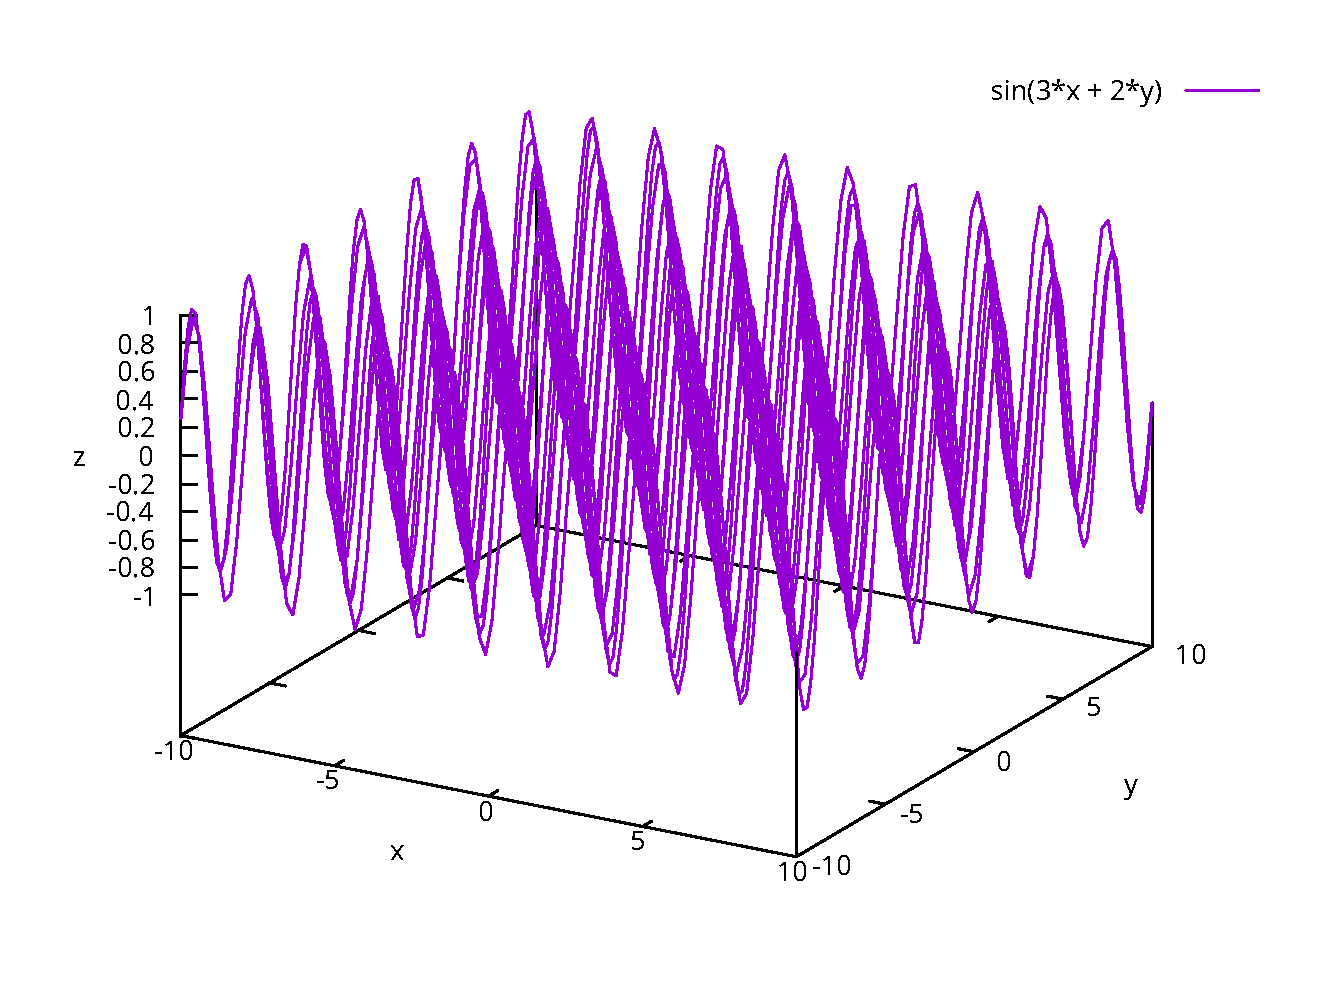
\includegraphics[width=0.8\textwidth]{graphics/komplexerPlot.pdf}
    \caption{Dreidimensionale Abbildung der Funktion $f(x,y) = \sin(3x+2y)$}
    \label{fig:comlex-plot}
\end{figure}

\subsection{Komplexe abgesetzte mathematische Formeln}

$$\int_1^3{\int_2^1 \sum_{k=1}^{\infty} 9x^iy^{i-1} dydx}$$

$$f(x) = a_0 + \sum_{n=1}^{\infty} (a_n\cos(\frac{n\pi x}{L}) + b_n\sin(\frac{n\pi x}{L}))$$

\subsection{Mathematische Formeln im Fließtext}

Lorem ipsum dolor sit amet $f(x) = 3x^2 + 2x - 5$, consetetur sapdisching elitr $f'(x)=5x+2$, sed diam nonumy eirmod tempo $\int_3^5 \frac{e^{f(x)}}{3} dx$.

\section{Anhang}

\subsection{Code zur Erzeugung von Abbildung \ref{fig:scherzo-amplitude}}

\textit{Shellskript zur Erzeugung der Audioamplitudendaten:}
\begin{lstlisting}
#!/usr/bin/bash
sox scherzo.wav -t dat - | tail -n +2 > amplitude.txt
\end{lstlisting}

\textit{Gnuplotskript zur Erzeugung des Amplitudenplots:}
\begin{lstlisting}
gnuplot> set xlabel "Zeit"
gnuplot> set ylabel "Amplitude"
gnuplot> plot "amplitude.txt" using 1:2 with lines title "Beethoven Symphony No.9 (Amplitudendarstellung)"
\end{lstlisting}

\subsection{Code zur Erzeugung von Abbildung \ref{fig:scherzo-frequenz}}

\textit{Pythonskript zur Erzeugung der Fourier Transformationsdaten:}
\begin{lstlisting}
import numpy as np 
from scipy.io import wavfile

rate, data = wavfile.read("scherzo.wav")
fft = np.fft.fft(data)
freqs = np.fft.fftfreq(len(fft), 1/rate)

if data.ndim > 1:
  data = data[:,0]
  fft = np.fft.fft(data)
  freqs = np.fft.fftfreq(len(fft), 1 / rate)

idx = np.where(freqs >= 0)

with open("fft_data.dat", "w") as f:
  for fval, amp in zip(freqs[idx], np.abs(fft[idx])):
    f.write(f"{fval}\t{amp}\n")
\end{lstlisting}

\textit{Gnuplotskript zur Erzeugung des Frequenzplots:}
\begin{lstlisting}
gnuplot> set xlabel "Frequenz"
gnuplot> set ylabel "Amplitude"
gnuplot> plot "fft_data,dat" using 1:2 with lines title "Beethoven Symphony No.9 (Frequenzdarstellung)"
\end{lstlisting}

\newpage

\subsection{Gnuplotskript zur Erzeugung von Abbildung \ref{fig:comlex-plot}}
\begin{lstlisting}
gnuplot> set xlabel "x"
gnuplot> set ylabel "y"
gnuplot> set zlabel "z"
gnuplot> splot sin(3*x + 2*y)
\end{lstlisting}

% Hier beginnt das Literaturverzeichnis
\clearpage
\renewcommand\refname{Literaturverzeichnis}
\bibliographystyle{alpha}
\bibliography{literatur}
\addcontentsline{toc}{section}{Literaturverzeichnis}


% Hier beginnt der Anhang
\clearpage


\end{document}
